% Options for packages loaded elsewhere
\PassOptionsToPackage{unicode}{hyperref}
\PassOptionsToPackage{hyphens}{url}
\PassOptionsToPackage{dvipsnames,svgnames,x11names}{xcolor}
%
\documentclass[
  11pt,
]{article}

\usepackage{amsmath,amssymb}
\usepackage{iftex}
\ifPDFTeX
  \usepackage[T1]{fontenc}
  \usepackage[utf8]{inputenc}
  \usepackage{textcomp} % provide euro and other symbols
\else % if luatex or xetex
  \usepackage{unicode-math}
  \defaultfontfeatures{Scale=MatchLowercase}
  \defaultfontfeatures[\rmfamily]{Ligatures=TeX,Scale=1}
\fi
\usepackage{lmodern}
\ifPDFTeX\else  
    % xetex/luatex font selection
    \setmainfont[]{Times New Roman}
\fi
% Use upquote if available, for straight quotes in verbatim environments
\IfFileExists{upquote.sty}{\usepackage{upquote}}{}
\IfFileExists{microtype.sty}{% use microtype if available
  \usepackage[]{microtype}
  \UseMicrotypeSet[protrusion]{basicmath} % disable protrusion for tt fonts
}{}
\makeatletter
\@ifundefined{KOMAClassName}{% if non-KOMA class
  \IfFileExists{parskip.sty}{%
    \usepackage{parskip}
  }{% else
    \setlength{\parindent}{0pt}
    \setlength{\parskip}{6pt plus 2pt minus 1pt}}
}{% if KOMA class
  \KOMAoptions{parskip=half}}
\makeatother
\usepackage{xcolor}
\usepackage[margin=1in]{geometry}
\setlength{\emergencystretch}{3em} % prevent overfull lines
\setcounter{secnumdepth}{-\maxdimen} % remove section numbering
% Make \paragraph and \subparagraph free-standing
\makeatletter
\ifx\paragraph\undefined\else
  \let\oldparagraph\paragraph
  \renewcommand{\paragraph}{
    \@ifstar
      \xxxParagraphStar
      \xxxParagraphNoStar
  }
  \newcommand{\xxxParagraphStar}[1]{\oldparagraph*{#1}\mbox{}}
  \newcommand{\xxxParagraphNoStar}[1]{\oldparagraph{#1}\mbox{}}
\fi
\ifx\subparagraph\undefined\else
  \let\oldsubparagraph\subparagraph
  \renewcommand{\subparagraph}{
    \@ifstar
      \xxxSubParagraphStar
      \xxxSubParagraphNoStar
  }
  \newcommand{\xxxSubParagraphStar}[1]{\oldsubparagraph*{#1}\mbox{}}
  \newcommand{\xxxSubParagraphNoStar}[1]{\oldsubparagraph{#1}\mbox{}}
\fi
\makeatother


\providecommand{\tightlist}{%
  \setlength{\itemsep}{0pt}\setlength{\parskip}{0pt}}\usepackage{longtable,booktabs,array}
\usepackage{calc} % for calculating minipage widths
% Correct order of tables after \paragraph or \subparagraph
\usepackage{etoolbox}
\makeatletter
\patchcmd\longtable{\par}{\if@noskipsec\mbox{}\fi\par}{}{}
\makeatother
% Allow footnotes in longtable head/foot
\IfFileExists{footnotehyper.sty}{\usepackage{footnotehyper}}{\usepackage{footnote}}
\makesavenoteenv{longtable}
\usepackage{graphicx}
\makeatletter
\newsavebox\pandoc@box
\newcommand*\pandocbounded[1]{% scales image to fit in text height/width
  \sbox\pandoc@box{#1}%
  \Gscale@div\@tempa{\textheight}{\dimexpr\ht\pandoc@box+\dp\pandoc@box\relax}%
  \Gscale@div\@tempb{\linewidth}{\wd\pandoc@box}%
  \ifdim\@tempb\p@<\@tempa\p@\let\@tempa\@tempb\fi% select the smaller of both
  \ifdim\@tempa\p@<\p@\scalebox{\@tempa}{\usebox\pandoc@box}%
  \else\usebox{\pandoc@box}%
  \fi%
}
% Set default figure placement to htbp
\def\fps@figure{htbp}
\makeatother

\makeatletter
\@ifpackageloaded{caption}{}{\usepackage{caption}}
\AtBeginDocument{%
\ifdefined\contentsname
  \renewcommand*\contentsname{Table of contents}
\else
  \newcommand\contentsname{Table of contents}
\fi
\ifdefined\listfigurename
  \renewcommand*\listfigurename{List of Figures}
\else
  \newcommand\listfigurename{List of Figures}
\fi
\ifdefined\listtablename
  \renewcommand*\listtablename{List of Tables}
\else
  \newcommand\listtablename{List of Tables}
\fi
\ifdefined\figurename
  \renewcommand*\figurename{Figure}
\else
  \newcommand\figurename{Figure}
\fi
\ifdefined\tablename
  \renewcommand*\tablename{Table}
\else
  \newcommand\tablename{Table}
\fi
}
\@ifpackageloaded{float}{}{\usepackage{float}}
\floatstyle{ruled}
\@ifundefined{c@chapter}{\newfloat{codelisting}{h}{lop}}{\newfloat{codelisting}{h}{lop}[chapter]}
\floatname{codelisting}{Listing}
\newcommand*\listoflistings{\listof{codelisting}{List of Listings}}
\makeatother
\makeatletter
\makeatother
\makeatletter
\@ifpackageloaded{caption}{}{\usepackage{caption}}
\@ifpackageloaded{subcaption}{}{\usepackage{subcaption}}
\makeatother

\usepackage{bookmark}

\IfFileExists{xurl.sty}{\usepackage{xurl}}{} % add URL line breaks if available
\urlstyle{same} % disable monospaced font for URLs
\hypersetup{
  pdftitle={The Relationship Between Life Expectancy and the Gini Coefficient},
  pdfauthor={Vishwamber Reddy; Cayou Shao; Hongyu Yin},
  colorlinks=true,
  linkcolor={blue},
  filecolor={Maroon},
  citecolor={Blue},
  urlcolor={Blue},
  pdfcreator={LaTeX via pandoc}}


\title{The Relationship Between Life Expectancy and the Gini
Coefficient}
\author{Vishwamber Reddy \and Cayou Shao \and Hongyu Yin}
\date{}

\begin{document}
\maketitle

\renewcommand*\contentsname{Table of contents}
{
\hypersetup{linkcolor=}
\setcounter{tocdepth}{3}
\tableofcontents
}

\subsubsection{Executive summary:}\label{executive-summary}

This study examines the relationship between income inequality and life
expectancy across nations from 1990 to 2020 using World Bank and Our
World in Data sources. Our analysis reveals a negative correlation
between income inequality (measured by the Gini coefficient) and life
expectancy, with more equitable societies generally experiencing longer
life spans.

While global life expectancy has increased over the study period, the
persistence of high inequality in certain regions continues to
correspond with lower life expectancy outcomes. These findings suggest
that addressing income inequality could be an important factor in
improving population health outcomes.

\subsubsection{Introduction:}\label{introduction}

The gap between rich and poor has become a defining challenge of our
time, with potential implications for population health that extend far
beyond economic considerations. While medical advances and improved
living standards have generally increased life expectancy worldwide, the
benefits of these improvements are not equally distributed. Recent
studies suggest that the degree of income inequality within a society
may play a crucial role in determining health outcomes.

Our investigation aims to contribute to the ongoing debate about whether
more equitable societies tend to be healthier societies, and what this
might mean for public policy. Understanding these patterns is essential
for policymakers seeking to improve both economic and health outcomes in
their communities.

\subsubsection{Research Question}\label{research-question}

Primary Research Question:

\begin{itemize}
\tightlist
\item
  What is the relationship between income inequality and life expectancy
  across different countries between 1990-2020?
\end{itemize}

Secondary Research Questions:

\begin{enumerate}
\def\labelenumi{\arabic{enumi}.}
\item
  How has the correlation between income inequality and life expectancy
  changed over the three-decade period?
\item
  Do countries with similar Gini coefficients show comparable life
  expectancy patterns regardless of their geographical location?
\end{enumerate}

\subsubsection{Methodology:}\label{methodology}

To investigate the relationship between income inequality and life
expectancy, we analyzed data from two primary sources: life expectancy
data from Our World in Data and Gini coefficient data from the World
Bank. The analysis focused on the period from 1990 to 2020, covering
multiple countries worldwide.

The Gini coefficient, ranging from 0 to 1, measures income inequality
within countries, where 0 represents perfect equality and 1 represents
maximum inequality. Life expectancy at birth represents the average
number of years a newborn would live under current mortality rates.

We performed the following data processing and analysis steps:

\begin{enumerate}
\def\labelenumi{\arabic{enumi}.}
\item
  Data cleaning by removing missing values and standardizing country
  names
\item
  Merging the datasets based on country and year
\item
  Computing summary statistics and correlation analysis
\item
  Creating visualizations to examine relationships and trends
\end{enumerate}

The cross-sectional analysis examined the relationship between life
expectancy and Gini coefficient at select years. The longitudinal
analysis tracked changes in both variables across time.

Table and Figure References:

As shown in Table 1, the average life expectancy was 72.82 years (SD =
7.84), and the average Gini coefficient was 0.38 (SD = 0.09), reflecting
substantial variability across countries.

\begin{longtable}[]{@{}rrrr@{}}

\caption{\label{tbl-summary-stats}Summary statistics for life expectancy
and Gini coefficient (1990-2020)}

\tabularnewline

\toprule\noalign{}
Mean\_Life\_Expectancy & SD\_Life\_Expectancy & Mean\_Gini & SD\_Gini \\
\midrule\noalign{}
\endhead
\bottomrule\noalign{}
\endlastfoot
72.81685 & 7.835837 & 0.3756492 & 0.0881552 \\

\end{longtable}

Figure 1 illustrates trends over time, showing a steady increase in life
expectancy and a mild decline in income inequality from 1990 to 2020.

\begin{figure}

\centering{

\pandocbounded{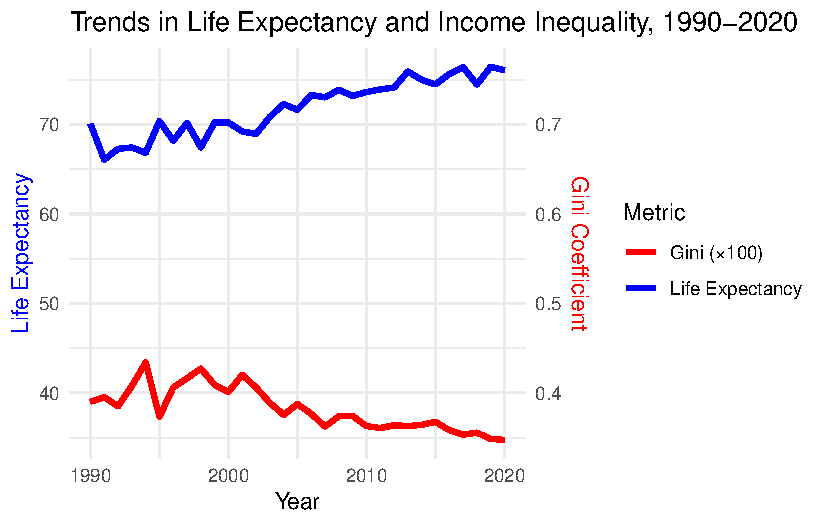
\includegraphics[keepaspectratio]{Assignment-3_files/figure-pdf/fig-time-trends-1.pdf}}

}

\caption{\label{fig-time-trends}Global trends in life expectancy and
Gini coefficient from 1990 to 2020}

\end{figure}%

\subsubsection{Results:}\label{results}

Our results demonstrate a negative correlation between income inequality
and life expectancy (r = -0.45). Countries with higher Gini coefficients
tend to have lower life expectancy.

Over the 30-year period, life expectancy increased globally from
approximately 70 years in 1990 to 76 years in 2020. Meanwhile, income
inequality slightly declined, with the average Gini coefficient
decreasing from 0.39 to 0.35.

Figure 2 presents cross-sectional snapshots by decade. The scatter plots
show a persistent negative relationship across time points, supporting
the association between inequality and health outcomes.

Notably, countries with Gini coefficients below 0.3 generally achieved
life expectancies above 80 years, while nations with coefficients above
0.45 frequently had life expectancies under 70 years.

The relationship remained consistent across decades, though the strength
of the correlation varied by region and development level. This suggests
that while income inequality is an important factor in life expectancy,
other variables likely play significant roles in determining population
health outcomes.

\begin{figure}

\centering{

\pandocbounded{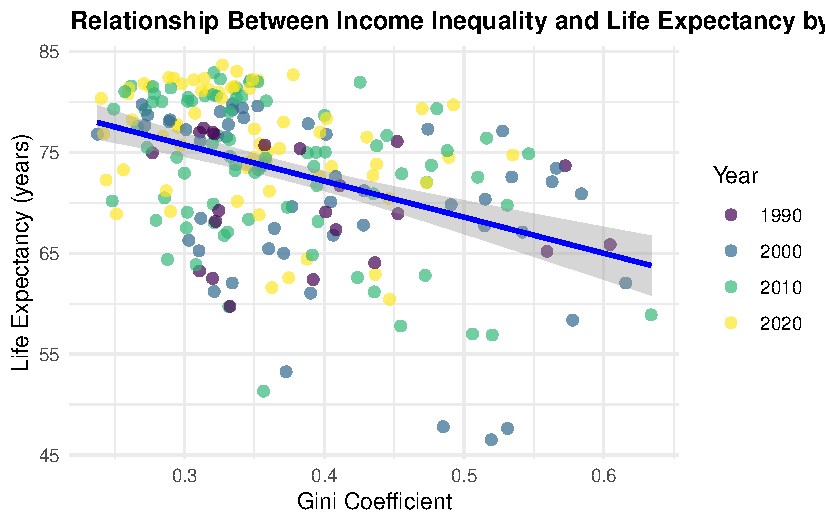
\includegraphics[keepaspectratio]{Assignment-3_files/figure-pdf/fig-scatter-decades-1.pdf}}

}

\caption{\label{fig-scatter-decades}Relationship between income
inequality and life expectancy}

\end{figure}%

\begin{figure}

\centering{

\pandocbounded{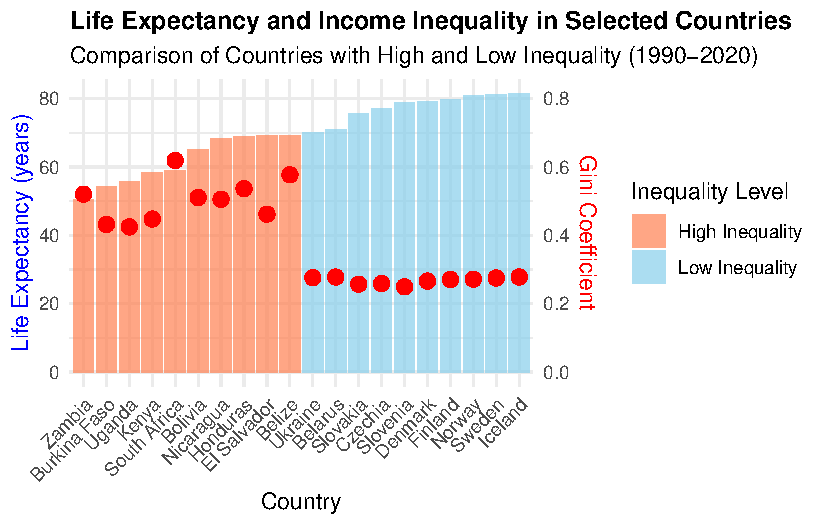
\includegraphics[keepaspectratio]{Assignment-3_files/figure-pdf/fig-country-comparison-1.pdf}}

}

\caption{\label{fig-country-comparison}Comparison of life expectancy and
income inequality}

\end{figure}%

\subsubsection{Discussion, conclusion and
recommendations}\label{discussion-conclusion-and-recommendations}

\subsubsection{Reference section:}\label{reference-section}

Include at least 1 reference.\\
\strut \\




\end{document}
